\documentclass[10pt]{beamer}
\usepackage[T2A]{fontenc}       %поддержка кириллицы
\usepackage[utf8]{inputenc}
\usepackage{lmodern}
\usepackage{scrextend}
\changefontsizes{16pt}
\usepackage{listings}
\usepackage{xcolor}
\graphicspath{{./images/}}
\usetheme{default}
\usecolortheme{crane}
\usefonttheme{structurebold}
\usefonttheme[onlymath]{serif}
\setbeamercovered{transparent}
\definecolor{name}{rgb}{0.5,0.5,0.5}
\begin{frame}{PHP}
  \begin{center}
    \begin{itemize}
      \item Interpretation
      \item Dynamic typing
      \item Garbage collector
      \item Procedure \& OOP
    \end{itemize}
  \end{center}
\end{frame}
\definecolor{mygray}{rgb}{0.5,0.5,0.5}
\definecolor{mymauve}{rgb}{0.58,0,0.82}
\definecolor{dkgreen}{rgb}{0,.6,0}
\definecolor{dkblue}{rgb}{0,0,.6}
\definecolor{dkyellow}{cmyk}{0,0,.8,.3}

\lstdefinestyle{htmlCode} {
   language=html,
   basicstyle=\tiny\ttfamily,
   keywordstyle=\ttfamily,
   commentstyle=\color{gray}\ttfamily,
   tabsize=1,
   frame=none,
   columns=fullflexible,
   escapechar=| % Escape to LaTeX between |...|
}
\begin{frame}{CSS}
CSS (Cascading Style Sheets) — формальный язык описания внешнего вида документа, написанного с использованием языка разметки.
\end{frame}
\begin{frame}[fragile]
 	\frametitle{CSS}
    \lstinputlisting[style=cssCode, linerange={9-11}, basicstyle=\footnotesize]{sources/code/html/class.css}
\end{frame}

% Set custom colors
\definecolor{code}{gray}{0}
\definecolor{canvas}{gray}{0.96}
\definecolor{comment}{rgb}{0, 0.456, 0}
\definecolor{keyword}{rgb}{0.5, 0, 0.5}

% JavaScript is not part of the listings package...
% but thankfully this page shows how to add it:
% http://lenaherrmann.net/2010/05/20/javascript-syntax-highlighting-in-the-latex-listings-package

\lstdefinelanguage{javascript}{
  keywords={typeof, new, true, false, catch, function, return, null, catch, switch, var, if, for, in, while, do, else, case, break},
  ndkeywords={class, export, boolean, throw, implements, import, this},
  sensitive=false,
  comment=[l]{//},
  morecomment=[s][\color{blue}\ttfamily]{/*}{*/},
  morestring=[b]',
  morestring=[b]"
}

% Parameters for formatting code (optional, affects all code listings)
\lstset{
  backgroundcolor=\color{canvas},
  basicstyle=\ttfamily\small\color{code},
  commentstyle=\color{comment},
  identifierstyle=\color{black},
  keywordstyle=\color{keyword}\bfseries,
  ndkeywordstyle=\color{keyword}\bfseries,
  stringstyle=\color{blue}\ttfamily
}

\lstdefinestyle{jsCode} {
   language=javascript,
   basicstyle=\tiny\ttfamily,
   keywordstyle=\ttfamily,
   commentstyle=\color{gray}\ttfamily,
   tabsize=1,
   frame=none,
   columns=fullflexible,
   escapechar=| % Escape to LaTeX between |...|
}
\definecolor{mygray}{rgb}{0.5,0.5,0.5}
\definecolor{mymauve}{rgb}{0.58,0,0.82}
\definecolor{dkgreen}{rgb}{0,.6,0}
\definecolor{dkblue}{rgb}{0,0,.6}
\definecolor{dkyellow}{cmyk}{0,0,.8,.3}

\lstdefinestyle{pascalCode} {
   language=pascal,
   basicstyle=\tiny\ttfamily,
   keywordstyle=\ttfamily,
   commentstyle=\color{gray}\ttfamily,
   tabsize=1,
   frame=none,
   columns=fullflexible,
   escapechar=| % Escape to LaTeX between |...|
}
\newcommand{\includecode}[2][c]{\lstinputlisting[caption=#2, escapechar=, style=custom#1]{#2}}


\title[Web]{Web программирование}
\subtitle[Web apps]{Web applications}
\author[Родионов И.Н.]{Игорь Родионов}
\institute[ОмГТУ ИВТ]{Омский Государственный Технический Университет\\
	{\tiny кафедра Информатики и вычислительной техники}\\
}
\date[2014]{ОмГТУ, 2014.}

\begin{document}
\begin{frame}[plain]
\maketitle
\end{frame}

\begin{frame}{Main Rule}
  \LARGE
  \begin{center}
    НЕ ДОВЕРЯЙТЕ ВХОДНЫМ ДАННЫМ
  \end{center}
\end{frame}
\begin{frame}[fragile]{Concurrency}
    \begin{columns}[t] % contents are top vertically aligned
         \begin{column}[T]{5cm} % each column can also be its own environment
            \begin{center}
              
\includegraphics[width=\textwidth,keepaspectratio]{sources/images/etot-nelovkiy-moment_9027667_big_.png}
            \end{center}
         \end{column}
         \begin{column}[T]{5cm} % alternative top-align that's better for graphics
            \begin{center}
            Этот неловкий момент, когда для объяснения материала курса, надо рассказать другой курс.
            \end{center}
         \end{column}
     \end{columns}
\end{frame}

\begin{frame}{3-thier architecture}
  \begin{center}
    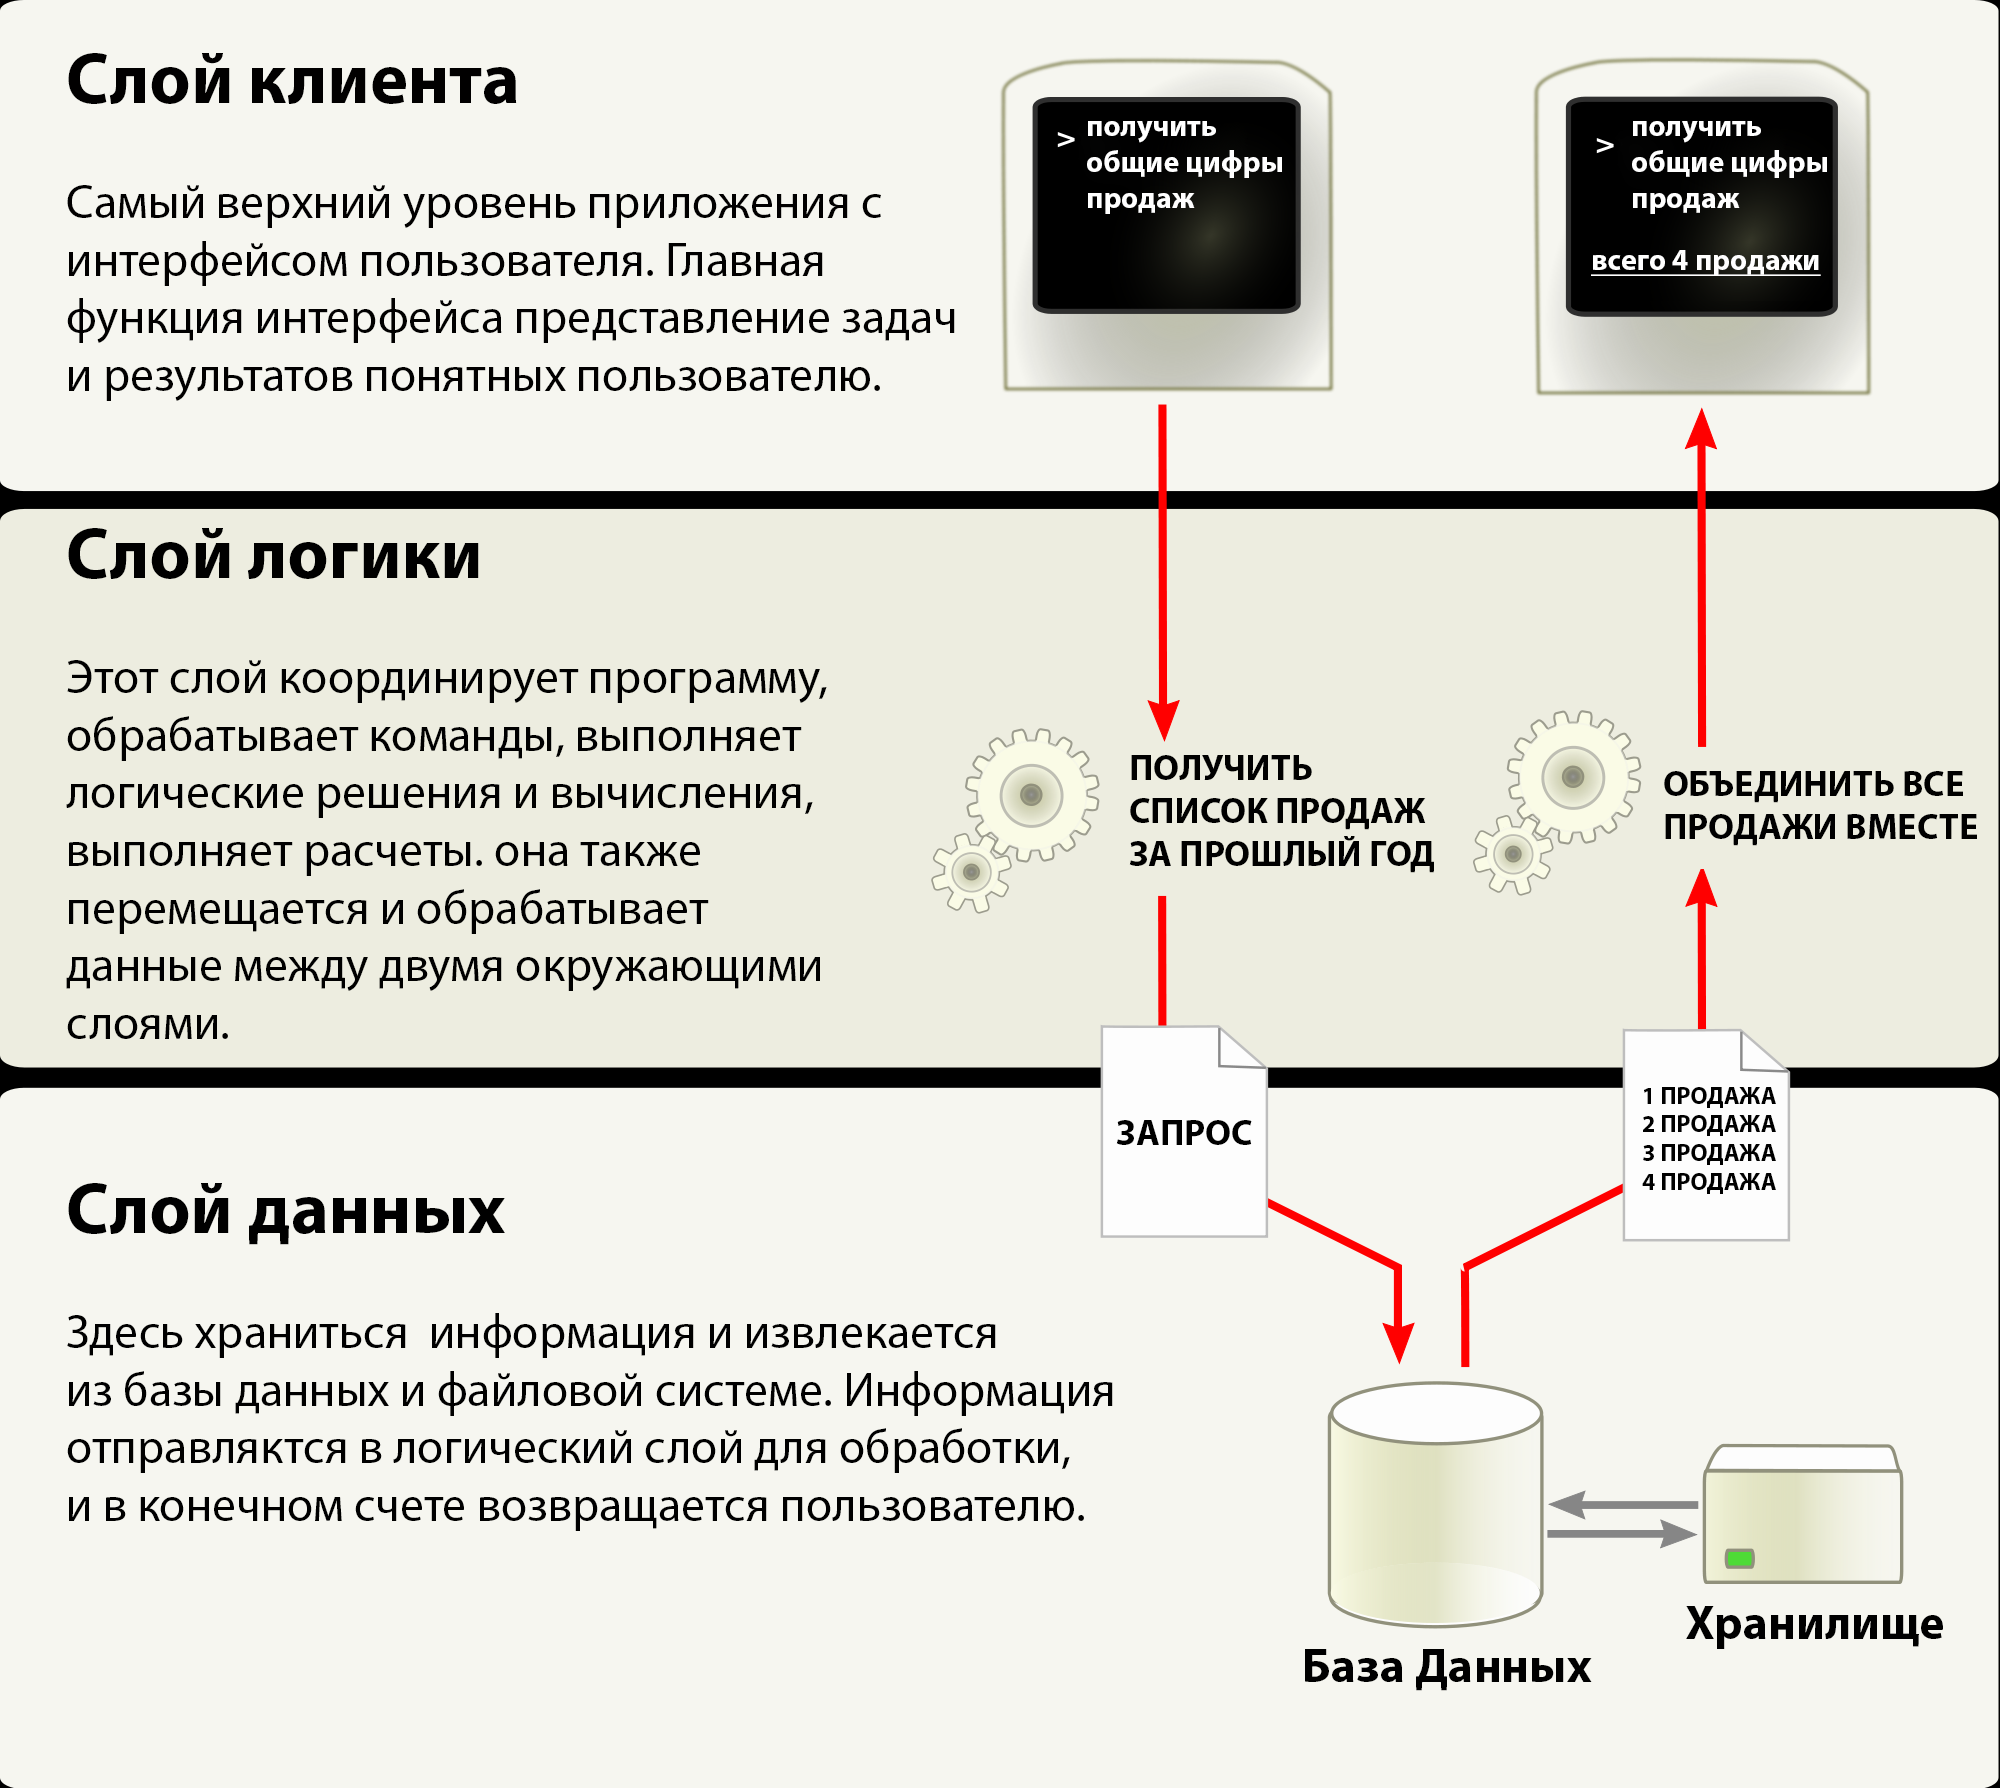
\includegraphics[height=7cm,keepaspectratio]{sources/images/CSD_SCHEME.png}
  \end{center}
\end{frame}
\begin{frame}{Questions}
 \begin{center}
    {\LARGE Вопросы?}
 \end{center}
\end{frame}
\begin{frame}{Systems}
  \begin{center}
    \begin{itemize}
      \item HTTP abstraction
      \item Session management
      \item Routing
      \item Data storage operations
      \item Business logic
      \item Templates
    \end{itemize}
  \end{center}
\end{frame}
\begin{frame}[fragile]{Concurrency}
    \begin{columns}[t] % contents are top vertically aligned
         \begin{column}[T]{5cm} % each column can also be its own environment
            \begin{center}
              
\includegraphics[width=\textwidth,keepaspectratio]{sources/images/etot-nelovkiy-moment_9027667_big_.png}
            \end{center}
         \end{column}
         \begin{column}[T]{5cm} % alternative top-align that's better for graphics
            \begin{center}
            Этот неловкий момент, когда для объяснения материала курса, надо рассказать другой курс.
            \end{center}
         \end{column}
     \end{columns}
\end{frame}

\begin{frame}{Systems}
  \begin{center}
    \begin{itemize}
      \item Compilation / Interpretation
      \item Static / Dynamic typing
      \item Memory management
      \item Programming paradigm
    \end{itemize}
  \end{center}
\end{frame}
\begin{frame}{PHP}
  \begin{center}
    \begin{itemize}
      \item Interpretation
      \item Dynamic typing
      \item Garbage collector
      \item Procedure \& OOP
    \end{itemize}
  \end{center}
\end{frame}
\definecolor{mygray}{rgb}{0.5,0.5,0.5}
\definecolor{mymauve}{rgb}{0.58,0,0.82}
\definecolor{dkgreen}{rgb}{0,.6,0}
\definecolor{dkblue}{rgb}{0,0,.6}
\definecolor{dkyellow}{cmyk}{0,0,.8,.3}

\lstdefinestyle{rubyCode} {
   language=Ruby,
   basicstyle=\tiny\ttfamily,
   keywordstyle=\ttfamily,
   commentstyle=\color{gray}\ttfamily,
   tabsize=1,
   frame=none,
   columns=fullflexible,
   escapechar=| % Escape to LaTeX between |...|
}
\begin{frame}{Node js}
  \begin{center}
    \begin{itemize}
      \item Interpretation
      \item Dynamic typing
      \item Garbage collector
      \item Procedure \& OOP \& Functional
    \end{itemize}
  \end{center}
\end{frame}
\definecolor{mygray}{rgb}{0.5,0.5,0.5}
\definecolor{mymauve}{rgb}{0.58,0,0.82}
\definecolor{dkgreen}{rgb}{0,.6,0}
\definecolor{dkblue}{rgb}{0,0,.6}
\definecolor{dkyellow}{cmyk}{0,0,.8,.3}

\lstdefinestyle{javaCode} {
   language=java,
   basicstyle=\tiny\ttfamily,
   keywordstyle=\ttfamily,
   commentstyle=\color{gray}\ttfamily,
   tabsize=1,
   frame=none,
   columns=fullflexible,
   escapechar=| % Escape to LaTeX between |...|
}
\begin{frame}{Systems}
  \begin{center}
    \begin{itemize}
      \item HTTP abstraction
      \item Session management
      \item Routing
      \item Data storage operations
      \item Business logic
      \item Templates
    \end{itemize}
  \end{center}
\end{frame}
\begin{frame}{Questions}
 \begin{center}
    {\LARGE Вопросы?}
 \end{center}
\end{frame}
\begin{frame}[fragile]{HTTP Abstraction - PHP}
  \begin{center}
    \lstinputlisting[style=phpCode, linerange={1-11}, basicstyle=\scriptsize]{sources/code/webapps/http.php}
  \end{center}
\end{frame}
\begin{frame}[fragile]{HTTP Abstraction - PHP}
  \begin{center}
    \lstinputlisting[style=phpCode, linerange={12-17}, basicstyle=\scriptsize]{sources/code/webapps/http.php}
  \end{center}
\end{frame}

\begin{frame}[fragile]{HTTP Abstraction - Ruby}
  \begin{center}
    \lstinputlisting[style=rubyCode, basicstyle=\scriptsize]{sources/code/webapps/rack.rb}
  \end{center}
\end{frame}

\begin{frame}[fragile]{HTTP Abstraction - Ruby}
  \begin{center}
    
\includegraphics[width=\textwidth,keepaspectratio]{sources/images/rack-logo.png}
  \end{center}
\end{frame}

\begin{frame}[fragile]{HTTP Abstraction - Ruby}
  \begin{center}
    \lstinputlisting[style=rubyCode, basicstyle=\scriptsize]{sources/code/webapps/rack_inside.rb}
  \end{center}
\end{frame}


\begin{frame}[fragile]{HTTP Abstraction - Node js}
  \begin{center}
    \lstinputlisting[style=jsCode, basicstyle=\scriptsize]{sources/code/webapps/node.js}
  \end{center}
\end{frame}


\begin{frame}[fragile]{HTTP Abstraction - Java}
  \begin{center}
    \lstinputlisting[style=javaCode, linerange={11-20}, basicstyle=\scriptsize]{sources/code/webapps/http.java}
  \end{center}
\end{frame}
\begin{frame}{Questions}
 \begin{center}
    {\LARGE Вопросы?}
 \end{center}
\end{frame}
\begin{frame}[fragile]{Session - PHP}
  \begin{center}
    \lstinputlisting[style=phpCode, basicstyle=\scriptsize]{sources/code/webapps/session.php}
  \end{center}
\end{frame}


\begin{frame}[fragile]{Session - Java}
  \begin{center}
    \lstinputlisting[style=javaCode, linerange={7-22, 35-36},  basicstyle=\tiny]{sources/code/webapps/session.java}
  \end{center}
\end{frame}



\begin{frame}{Questions}
 \begin{center}
    {\LARGE Вопросы?}
 \end{center}
\end{frame}
\begin{frame}[fragile]{Concurrency}
    \begin{columns}[t] % contents are top vertically aligned
         \begin{column}[T]{5cm} % each column can also be its own environment
            \begin{center}
              
\includegraphics[width=\textwidth,keepaspectratio]{sources/images/etot-nelovkiy-moment_9027667_big_.png}
            \end{center}
         \end{column}
         \begin{column}[T]{5cm} % alternative top-align that's better for graphics
            \begin{center}
            Этот неловкий момент, когда для объяснения материала курса, надо рассказать другой курс.
            \end{center}
         \end{column}
     \end{columns}
\end{frame}

\begin{frame}[fragile]{Model View Controller}
  \begin{center}
    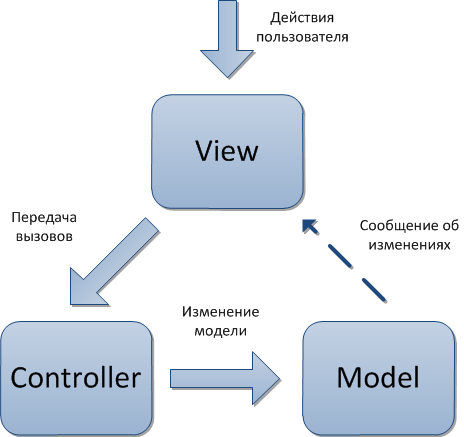
\includegraphics[height=7cm,keepaspectratio]{sources/images/mvc.png}
  \end{center}
\end{frame}
\begin{frame}[fragile]{Model View Presenter}
  \begin{center}
    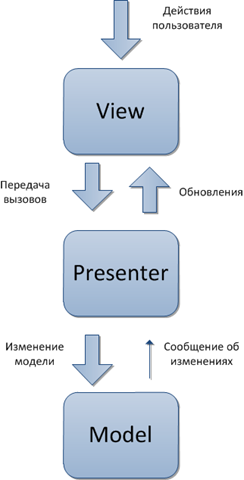
\includegraphics[height=7cm,keepaspectratio]{sources/images/mvp.png}
  \end{center}
\end{frame}
\begin{frame}[fragile]{MVC - PHP}
  \begin{center}
    \lstinputlisting[style=phpCode, linerange={2-22}, basicstyle=\tiny]{sources/code/webapps/mvc.php}
  \end{center}
\end{frame}



\begin{frame}{Questions}
 \begin{center}
    {\LARGE Вопросы?}
 \end{center}
\end{frame}
\begin{frame}[fragile]{MVC - PHP}
  \begin{center}
    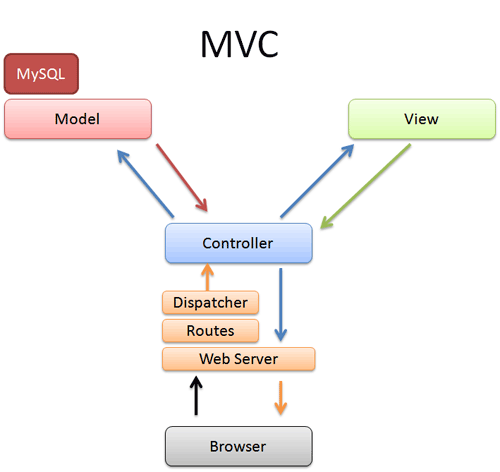
\includegraphics[height=7cm, keepaspectratio]{sources/images/mvc-in-php.png}
  \end{center}
\end{frame}
\begin{frame}[fragile]{Routing}
  \begin{center}
    \scriptsize
    \begin{verbatim}
http://site.com/shop/computers - категория "Компьютеры"
http://site.com/shop/computers/23 - товар с ID = 23
    \end{verbatim}
        \begin{verbatim}
'shop/category/<category:[\w_\/-]+>/<id:[\d]+>'=>'shop/show',
'shop/category/<category:[\w_\/-]+>'=>'shop/category',
'shop'=>'shop/index',
        \end{verbatim}
  \end{center}
\end{frame}

\begin{frame}[fragile]{Routing}
  \begin{center}
    \lstinputlisting[style=phpCode, basicstyle=\tiny]{sources/code/webapps/controller.php}
  \end{center}
\end{frame}



\begin{frame}{Questions}
 \begin{center}
    {\LARGE Вопросы?}
 \end{center}
\end{frame}
\begin{frame}[fragile]{MVC - PHP}
  \begin{center}
    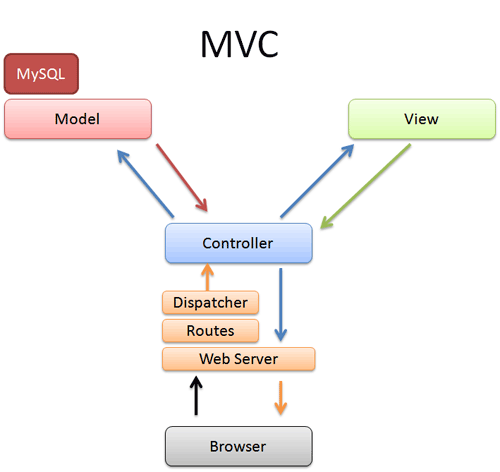
\includegraphics[height=7cm, keepaspectratio]{sources/images/mvc-in-php.png}
  \end{center}
\end{frame}
\begin{frame}[fragile]{Model - ORM}
  \begin{center}
    \lstinputlisting[style=rubyCode, basicstyle=\tiny]{sources/code/webapps/activerecord.rb}
  \end{center}
\end{frame}

\begin{frame}[fragile]{Model View Controller}
  \begin{center}
    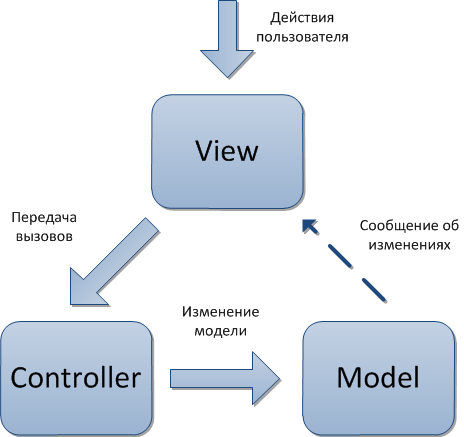
\includegraphics[height=7cm,keepaspectratio]{sources/images/mvc.png}
  \end{center}
\end{frame}
\begin{frame}[fragile]{View - Templates}
  \begin{center}
    \lstinputlisting[style=phpCode, basicstyle=\tiny]{sources/code/webapps/smarty.php}
  \end{center}
\end{frame}

\begin{frame}[fragile]{View - Templates}
  \begin{center}
    \lstinputlisting[style=htmlCode, basicstyle=\tiny]{sources/code/webapps/smarty.tpl}
  \end{center}
\end{frame}

\begin{frame}{Questions}
 \begin{center}
    {\LARGE Вопросы?}
 \end{center}
\end{frame}
\end{document}

